\documentclass[12pt]{article}

\usepackage{color}
\usepackage{amsmath}
\usepackage{amssymb}
\usepackage{latexsym}
\usepackage{amsfonts}
%\usepackage{times}
\usepackage{url}
%\usepackage{bibspacing}
%\setlength{\bibspacing}{\baselineskip}
\usepackage{hyperref}
\usepackage{xspace}
\usepackage{graphicx}
\usepackage{caption}
\usepackage{subcaption}
\marginparwidth 5pt \oddsidemargin  2pt \evensidemargin  2pt
\marginparsep 0pt
\topmargin   -40pt
\textwidth   6.5in \textheight  9 in


\begin{document}

\section{IPSec}
IP-level security encompasses three functional areas: authentication, confidentiality, and key management. The authentication mechanism assures that a received packet was, in fact, transmitted by the party identified as the source in the packet header. In addition, this mechanism assures that the packet has not been altered in transit. The confidentiality facility enables communicating nodes to encrypt messages to prevent eavesdropping by third parties. The key management facility is concerned with the secure exchange of keys.

The principal feature of IPSec that enables it to support these varied applications is that it can encrypt and/or authenticate all traffic at the IP level. Thus, all distributed applications, including remote logon, client/server, e-mail, file transfer, Web access, and so on, can be secured.

A key concept that appears in both the authentication and confidentiality mechanisms for IP is the security association (SA). An association is a one-way relationship between a sender and a receiver that affords security services to the traffic carried on it. If a peer relationship is needed, for two-way secure exchange, then two security associations are required. Security services are afforded to an SA for the use of AH or ESP, but not both.

A security association is uniquely identified by three parameters:
\begin{description}
\item[Security Parameters Index (SPI)] A bit string assigned to this SA and having local significance only. The SPI is carried in AH and ESP headers to enable the receiving system to select the SA under which a received packet will be processed.
\item[IP Destination Address] Currently, only unicast addresses are allowed; this is the address of the destination endpoint of the SA, which may be an end user system or a network system such as a firewall or router.
\item[Security Protocol Identifier] This indicates whether the association is an AH or ESP security association.
\end{description}

There are two main wire-level protocols used by IPSec, AH (Authentication Header) and ESP (Encapsulating Security Payload), and they authenticate (AH) and encrypt optionally) (ESP which can optionally also authenticate) the data flowing over that connection. They are typically used independently, though it's possible (but uncommon) to use them both together.

Both of the above protocols can be deployed in two distinct modes, Transport mode and Tunnel mode. Transport Mode provides a secure connection between two endpoints as it encapsulates IP's payload, while Tunnel Mode encapsulates the entire IP packet to provide a virtual "secure hop" between two gateways. The latter is used to form a traditional VPN, where the tunnel generally creates a secure tunnel across an untrusted Internet.

\subsection*{Authenticated Header}

AH is used to authenticate — but not encrypt — IP traffic, and this serves the treble purpose of ensuring that we're really talking to who we think we are, detecting alteration of data while in transit, and (optionally) to guard against replay by attackers who capture data from the wire and attempt to re-inject that data back onto the wire at a later date.
Authentication is performed by computing a cryptographic hash-based message authentication code over nearly all the fields of the IP packet (excluding those which might be modified in transit, such as TTL or the header checksum), and stores this in a newly-added AH header and sent to the other end.
 
This AH header contains just five interesting fields, and it's injected between the original IP header and the payload. We'll touch on each of the fields here, though their utility may not be fully apparent until we see how they're used in the larger picture.

\begin{description}
\item[next hdr]
This identifies the protocol type of the following payload, and it's the original packet type being encapsulated: this is how the IPsec header(s) are linked together.
\item[AH len]
This defines the length, in 32-bit words, of the whole AH header, minus two words (this "minus two words" proviso springs from the format of IPv6's RFC 1883 Extension Headers, of which AH is one).
\item[Reserved]
This field is reserved for future use and must be zero.
\item[Security Parameters Index]
This is an opaque 32-bit identifier that helps the recipient select which of possibly many ongoing conversations this packet applies. Each AH-protected connection implies a hash algorithm (MD5, SHA-1, etc.), some kind of secret data, and a host of other parameters. The SPI can be thought of as an index into a table of these settings, allowing for easy association of packet with parameter.
\item[Sequence Number]
This is a monotonically increasing identifier that's used to assist in antireplay protection. This value is included in the authentication data, so modifications (intentional or otherwise) are detected.
\item[Authentication Data]
This is the Integrity Check Value calculated over the entire packet — including most of the headers — The recipient recomputes the same hash; Mismatched values mark the packet as either damaged in transit, or not having the proper secret key. These are discarded.
\end{description}

\paragraph{Transport Mode}
In AH Transport Mode, the IP packet is modified only slightly to include the new AH header between the IP header and the protocol payload (TCP, UDP, etc.), and there is a shuffling of the protocol code that links the various headers together.
This protocol shuffling is required to allow the original IP packet to be reconstituted at the other end: after the IPsec headers have been validated upon receipt, they're stripped off, and the original protocol type (TCP, UDP, etc.) is stored back in the IP header. We'll see this chain of next header fields again and again as we examine IPsec.
When the packet arrives at its destination and passes the authentication check, the AH header is removed and the Proto=AH field in the IP header is replaced with the saved "Next Protocol". This puts the IP datagram back to its original state, and it can be delivered to the waiting process.

\paragraph{Tunnel Mode}
Like Transport mode, the packet is sealed with an Integrity Check Value to authenticate the sender and to prevent modification in transit. But unlike Transport mode, it encapsulates the full IP header as well as the payload, and this allows the source and destination addresses to be different from those of the encompassing packet: This allows formation of a tunnel.

When a Tunnel-mode packet arrives at its destination, it goes through the same authentication check as any AH-type packet, and those passing the check have their entire IP and AH headers stripped off. This effectively reconstitutes the original IP datagram, which is then injected into the usual routing process.
Most implementations treat the Tunnel-mode endpoint as a virtual network interface — just like an Ethernet interface or localhost — and the traffic entering or leaving it is subject to all the ordinary routing decisions.
The reconstituted packet could be delivered to the local machine or routed elsewhere (according to the destination IP address found in the encapsulated packet), though in any case is no longer subject to the protections of IPsec. At this point, it's just a regular IP datagram.
Though Transport mode is used strictly to secure an end-to-end connection between two computers, Tunnel mode is more typically used between gateways (routers, firewalls, or standalone VPN devices) to provide a Virtual Private Network (VPN).
 
\begin{figure}[h!]
        \centering
        \begin{subfigure}[b]{0.45\textwidth}
                \centering
                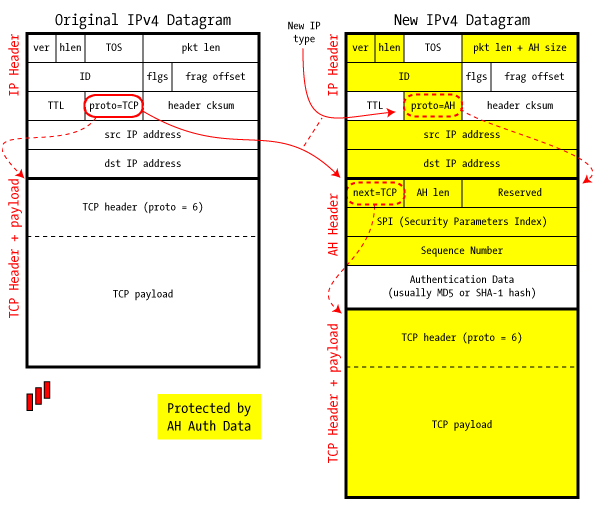
\includegraphics[width=\textwidth]{AH-1.png}
                \caption{Transport Mode}
                \end{subfigure}
        \qquad
        \begin{subfigure}[b]{0.45\textwidth}
                \centering
                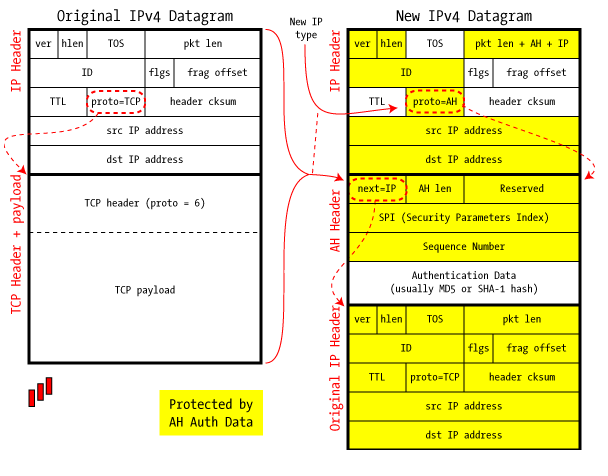
\includegraphics[width=\textwidth]{AH-2.png}
                \caption{Tunnel Mode}
                \end{subfigure}
        \caption{Authenticated Header mode}
\end{figure}

\subsection{Encapsulating Security Payload}
Adding encryption makes ESP a bit more complicated because the encapsulation surrounds the payload rather than precedes it as with AH: ESP includes header and trailer fields to support the encryption and optional authentication. It also provides Tunnel and Transport modes which are used in by-now familiar ways.
The IPsec RFCs don't insist upon any particular encryption algorithms, but we find DES, triple-DES, AES, and Blowfish in common use to shield the payload from prying eyes. The algorithm used for a particular connection is specified by the Security Association (covered in a later section), and this SA includes not only the algorithm, but the key used.
Unlike AH, which provides a small header before the payload, ESP surrounds the payload it's protecting. The Security Parameters Index and Sequence Number serve the same purpose as in AH, but we find padding, the next header, and the optional Authentication Data at the end, in the ESP Trailer.
It's possible to use ESP without any actual encryption (to use a NULL algorithm), which nonetheless structures the packet the same way. This provides no confidentiality, and it only makes sense if combined with ESP authentication. It's pointless to use ESP without either encryption or authentication (unless one is simply doing protocol testing).
Padding is provided to allow block-oriented encryption algorithms room for multiples of their blocksize, and the length of that padding is provided in the pad len field. The next hdr field gives the type (IP, TCP, UDP, etc.) of the payload in the usual way, though it can be thought of as pointing "backwards" into the packet rather than forward as we've seen in AH.

In addition to encryption, ESP can also optionally provide authentication, with the same HMAC as found in AH. Unlike AH, however, this authentication is only for the ESP header and encrypted payload: it does not cover the full IP packet. Surprisingly, this does not substantially weaken the security of the authentication, but it does provide some important benefits.
When an outsider examines an IP packet containing ESP data, it's essentially impossible to make any real guesses about what's inside save for the usual data found in the IP header (particularly the source and destination IP addresses). The attacker will certainly know that it's ESP data — that's also in the header — but the type of the payload is encrypted with the payload.
Even the presence or absence of Authentication Data can't be determined by looking at the packet itself (this determination is made by using the Security Parameters Index to reference the preshared set of parameters and algorithms for this connection).
However, it should be noted that sometimes the envelope provides hints that the payload does not. With more people sending VoIP inside ESP over the internet, the QoS taggings are in the outside header and is fairly obvious what traffic is VoIP signaling (IP precedence 3) and what is RTP traffic (IP precedence 5). It's not a sure thing, but it might be enough of a clue to matter in some circumstances.

\paragraph{Transport Mode}
As with AH, Transport Mode encapsulates just the datagram's payload and is designed strictly for host-to-host communications. The original IP header is left in place (except for the shuffled Protocol field), and it means that — among other things — the source and destination IP addresses are unchanged.

Transport mode operation may be summarized as follows:
\begin{enumerate}
\item At the source, the block of data consisting of the ESP trailer plus the entire transport-layer segment is encrypted and the plaintext of this block is replaced with its ciphertext to form the IP packet for transmission. Authentication is added if this option is selected.
\item 
The packet is then routed to the destination. Each intermediate router needs to examine and process the IP header plus any plaintext IP extension headers but does not need to examine the ciphertext.
\item
The destination node examines and processes the IP header plus any plaintext IP extension headers. Then, on the basis of the SPI in the ESP header, the destination node decrypts the remainder of the packet to recover the plaintext transport-layer segment.
\end{enumerate}
Transport mode operation provides confidentiality for any application that uses it, thus avoiding the need to implement confidentiality in every individual application. This mode of operation is also reasonably efficient, adding little to the total length of the IP packet. One drawback to this mode is that it is possible to do traffic analysis on the transmitted packets.


\paragraph{Tunnel Mode}
Unlike AH, where an onlooker can easily tell whether traffic is in Tunnel or Transport mode, this information is unavailable here: the fact that this is Tunnel mode (via next=IP) is part of the encrypted payload, and is simply not visible to one unable to decrypt the packet.

Because the IP header contains the destination address and possibly source routing directives and hop- by-hop option information, it is not possible simply to transmit the encrypted IP packet prefixed by the ESP header. Intermediate routers would be unable to process such a packet. Therefore, it is necessary to encapsulate the entire block (ESP header plus ciphertext plus Authentication Data, if present) with a new IP header that will contain sufficient information for routing but not for traffic analysis.
Whereas the transport mode is suitable for protecting connections between hosts that support the ESP feature, the tunnel mode is useful in a configuration that includes a firewall or other sort of security gateway that protects a trusted network from external networks. In this latter case, encryption occurs only between an external host and the security gateway or between two security gateways. This relieves hosts on the internal network of the processing burden of encryption and simplifies the key distribution task by reducing the number of needed keys. Further, it thwarts traffic analysis based on ultimate destination.
Consider a case in which an external host wishes to communicate with a host on an internal network protected by a firewall, and in which ESP is implemented in the external host and the firewalls. The following steps occur for transfer of a transport-layer segment from the external host to the internal host:
\begin{enumerate}
\item
The source prepares an inner IP packet with a destination address of the target internal host. This packet is prefixed by an ESP header; then the packet and ESP trailer are encrypted and Authentication Data may be added. The resulting block is encapsulated with a new IP header (base header plus optional extensions such as routing and hop-by-hop options for IPv6) whose destination address is the firewall; this forms the outer IP packet.
\item 
The outer packet is routed to the destination firewall. Each intermediate router needs to examine and process the outer IP header plus any outer IP extension headers but does not need to examine the ciphertext.
\item
The destination firewall examines and processes the outer IP header plus any outer IP extension headers. Then, on the basis of the SPI in the ESP header, the destination node decrypts the remainder of the packet to recover the plaintext inner IP packet. This packet is then transmitted in the internal network.
\item The inner packet is routed through zero or more routers in the internal network to the destination host.
\end{enumerate}

\begin{figure}[h!]
        \centering
        \begin{subfigure}[b]{0.45\textwidth}
                \centering
                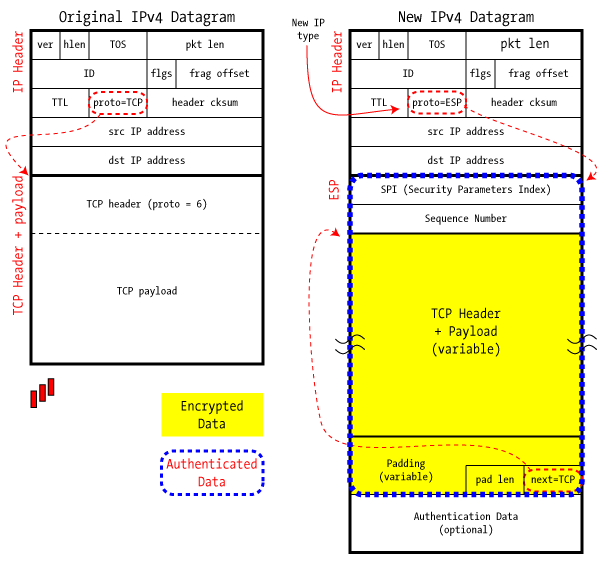
\includegraphics[width=\textwidth]{ESP-1.png}
                \caption{Transport Mode}
                \end{subfigure}
        \qquad
        \begin{subfigure}[b]{0.45\textwidth}
                \centering
                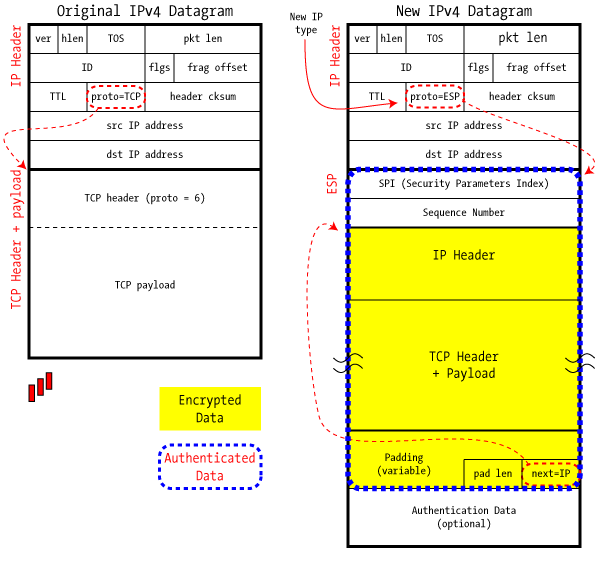
\includegraphics[width=\textwidth]{ESP-2.png}
                \caption{Tunnel Mode}
                \end{subfigure}
        \caption{Encapsulating Security Payload mode}
\end{figure}

\subsection{Combining Authentication and Encryption}
Encryption and authentication can be combined in order to transmit an IP packet that has both confidentiality and authentication between hosts. We know that ESP is the only way to provide encryption, but ESP and AH both can provide authentication: which one do we use?
 
The obvious solution of wrapping ESP inside of AH is technically possible, but in practice is not commonly used because of AH's limitations with respect to Network Address Translation. By using AH+ESP, this tunnel could never successfully traverse a NAT'ed device.

Instead, ESP+Auth is used in Tunnel mode to fully encapsulate the traffic on its way across an untrusted network, protected by both encryption and authentication in the same thing.
Traffic protected in this manner yields nearly no useful information to an interloper save for the fact that the two sites are connected by a VPN. This information might help an attacker understand trust relationships, but nothing about the actual traffic itself is revealed. Even the type of encapsulated protocol — TCP, UDP, or ICMP — is hidden from outsiders.
What's particularly nice about this mode of operation is that the end-user hosts generally know nothing about the VPN or other security measures in place. Since a VPN implemented by a gateway device treats the VPN as yet another interface, traffic destined for the other end is routed normally.
This packet-in-a-packet can actually be nested yet more levels: Host A and Host B can establish their own authenticated connection (via AH), and have this routed over the VPN. This would put an AH inner packet inside an enclosing ESP+Auth packet.

\begin{figure}
  \centering
  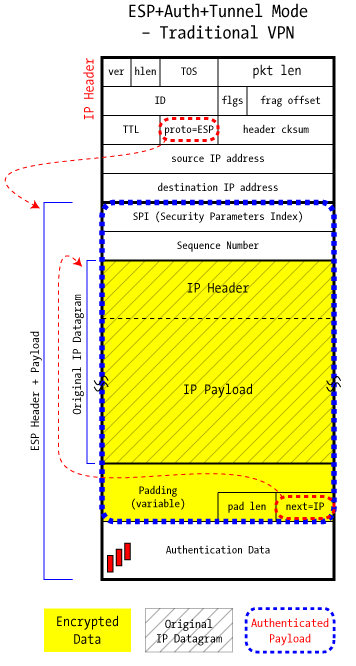
\includegraphics[scale = 0.5]{VPN.png}
  \caption{ESP + Authentication}
 \end{figure}

\subsection{General Remarks and Comments on IPSec}
\paragraph*{AH and NAT}
Though AH provides very strong protection of a packet's contents because it covers everything that can be possibly considered immutable, this protection comes at a cost: AH is incompatible with NAT (Network Address Translation).
 
NAT is used to map a range of private addresses (say, 192.168.1.X) to and from a (usually) smaller set of public address, thereby reducing the demand for routable, public IP space. In this process, the IP header is actually modified on the fly by the NAT device to change the source and/or destination IP address.
When the appropriate source or header IP address is changed, it forces a recalculation of the header checksum. This has to be done anyway, because the NAT device typically serves as one "hop" in the path from source to destination, and this requires the decrement of the TTL (Time To Live) field.
Because the TTL and header checksum fields are always modified in flight, AH knows to excludes them from coverage, but this does not apply to the IP addresses. These are included in the Integrity Check Value, and any modification will cause the check to fail when verified by the recipient. Because the ICV incorporates a secret key which is unknown by intermediate parties, the NAT router is not able to recompute the ICV.
This same difficulty also applies to PAT (Port Address Translation), which maps multiple private IP addresses into a single external IP address. Not only are the IP addresses modified on the fly, but the UDP and TCP port numbers (and sometimes even to payload). This requires much more intelligence on the part of the NAT device, and more extensive modifications to the whole IP datagram.


\paragraph*{Anti-Replay Mechanism}
A replay attack is one in which an attacker obtains a copy of an authenticated packet and later transmits it to the intended destination. The receipt of duplicate, authenticated IP packets may disrupt service in some way or may have some other undesired consequence. The Sequence Number field is designed to thwart such attacks. First, we discuss sequence number generation by the sender, and then we look at how it is processed by the recipient.


When a new SA is established, the sender initializes a sequence number counter to 0. Each time that a packet is sent on this SA, the sender increments the counter and places the value in the Sequence Number field. Thus, the first value to be used is 1. If anti-replay is enabled (the default), the sender must not allow the sequence number to cycle past 232 1 back to zero. Otherwise, there would be multiple valid packets with the same sequence number. If the limit of 232 1 is reached, the sender should terminate this SA and negotiate a new SA with a new key.

Because IP is a connectionless, unreliable service, the protocol does not guarantee that packets will be delivered in order and does not guarantee that all packets will be delivered. Therefore, the IPSec authentication document dictates that the receiver should implement a window of size W, with a default of W = 64. The right edge of the window represents the highest sequence number, N, so far received for a valid packet. For any packet with a sequence number in the range from N W + 1 to N that has been correctly received (i.e., properly authenticated), the corresponding slot in the window is marked (Figure 16.4). Inbound processing proceeds as follows when a packet is received:
\begin{enumerate}
\item
If the received packet falls within the window and is new, the MAC is checked. If the packet is authenticated, the corresponding slot in the window is marked.
\item
If the received packet is to the right of the window and is new, the MAC is checked. If the packet is authenticated, the window is advanced so that this sequence number is the right edge of the window, and the corresponding slot in the window is marked.
\item
If the received packet is to the left of the window, or if authentication fails, the packet is discarded; this is an auditable event.
\end{enumerate}

\paragraph*{Integrity Chech Value}
The Authentication Data field holds a value referred to as the Integrity Check Value. The ICV is a message authentication code or a truncated version of a code produced by a MAC algorithm. The current specification dictates that a compliant implementation must support HMAC-MD5-96 and HMAC-SHA-1-96
Both of these use the HMAC algorithm, the first with the MD5 hash code and the second with the SHA-1 hash code. In both cases, the full HMAC value is
calculated but then truncated by using the first 96 bits, which is the default length for the Authentication Data field.

The MAC is calculated over
\begin{itemize}
\item IP header fields that either do not change in transit (immutable) or that are predictable in value upon arrival at the endpoint for the AH SA. Fields that may change in transit and whose value on arrival are unpredictable are set to zero for purposes of calculation at both source and destination.
\item The AH header other than the Authentication Data field. The Authentication Data field is set to zero for purposes of calculation at both source and destination.
\item The entire upper-level protocol data, which is assumed to be immutable in transit (e.g., a TCP segment or an inner IP packet in tunnel mode).
\end{itemize}
For IPv4, examples of immutable fields are Internet Header Length and Source Address. An example of a mutable but predictable field is the Destination Address (with loose or strict source routing). Examples of mutable fields that are zeroed prior to ICV calculation are the Time to Live and Header Checksum fields. Note that both source and destination address fields are protected, so that address spoofing is prevented.

For IPv6, examples in the base header are Version (immutable), Destination Address (mutable but predictable), and Flow Label (mutable and zeroed for calculation).
\paragraph*{Encryption Algorithms}
The Payload Data, Padding, Pad Length, and Next Header fields are encrypted by the ESP service. If the algorithm used to encrypt the payload requires cryptographic synchronization data, such as an initialization vector (IV), then these data may be carried explicitly at the beginning of the Payload Data field. If included, an IV is usually not encrypted, although it is often referred to as being part of the ciphertext.
The current specification dictates that a compliant implementation must support DES in cipher block chaining (CBC) mode (described in Chapter 3). Other algorithms supported include:
\begin{itemize}
\item Three-key triple DES
\item RC5
\item IDEA
\item Three-key triple IDEA
\item CAST
\item Blowfish
\end{itemize}
\paragraph*{Padding}
The Padding field serves several purposes:
\begin{itemize}
\item If an encryption algorithm requires the plaintext to be a multiple of some number of bytes (e.g., the multiple of a single block for a block cipher), the Padding field is used to expand the plaintext (consisting of the Payload Data, Padding, Pad Length, and Next Header fields) to the required length.
\item The ESP format requires that the Pad Length and Next Header fields be right aligned within a 32- bit word. Equivalently, the ciphertext must be an integer multiple of 32 bits. The Padding field is used to assure this alignment.
\item Additional padding may be added to provide partial traffic flow confidentiality by concealing the actual length of the payload.
\end{itemize}
\paragraph*{Key-Exchange}
The key management portion of IPSec involves the determination and distribution of secret keys. A typical requirement is four keys for communication between two applications: transmit and receive pairs for both AH and ESP. The IPSec Architecture document mandates support for two types of key management:
\begin{itemize}

\item Manual: A system administrator manually configures each system with its own keys and with the keys of other communicating systems. This is practical for small, relatively static environments.
\item Automated: An automated system enables the on-demand creation of keys for SAs and facilitates the use of keys in a large distributed system with an evolving configuration.
\end{itemize}
The default automated key management protocol for IPSec is referred to as ISAKMP/Oakley and consists of the following elements:
\begin{enumerate}

\item Oakley Key Determination Protocol: Oakley is a key exchange protocol based on the Diffie- Hellman algorithm but providing added security. Oakley is generic in that it does not dictate specific formats.
\item Internet Security Association and Key Management Protocol (ISAKMP): ISAKMP provides a framework for Internet key management and provides the specific protocol support, including formats, for negotiation of security attributes.
\end{enumerate}

\section{S-BGP}
Internrnet routing is based on a distributed system composed of many routers, grouped into management domains called Autonomous Systems (ASes). Routing information
is exchanged between ASes using the Border Gateway Protoco(BGP).

\subsection{Overview of BGP}

Routers implementing BGP, BGP “speakers,” exchange routing information via UPDATE messages. An UPDATE message consists of three parts:
\begin{enumerate}
\item  alist of address prefixes
for destinations that are no longer reachable (via the previously specified route) 
\item a list of prefixes that
are reachable
\item the characteristics of the cumulative path and
current inter-AS hop, contained in path attributes, that can be
used to reach the address prefixes. 
\end{enumerate}

The attribute used to specify the inter-AS path, the AS\_PATH attribute, specifies a sequence
of Autonomous Systems (ASes) along the path, each identified
by its AS number.

When propagating an UPDATE to a neighboring AS, the BGP
speaker prepends its AS number to the sequence, and updates
certain other path attributes. 
The backbone routers of the major internet service providers
(ISP’s) have a route to every reachable IP address. 
Each (nonleaf) BGP speaker maintains a full routing table, and
sends its best route for each prefix to each neighbor speaker.
When a BGP speaker reboots, it receives complete routing tables (via UPDATE’s) from each of its neighbors. 

BGP is deployed over TCP/IP.

\subsection{BGP Exploits and Vulnerabilities}

An ideal execution of BGP satisfies the following constraints:
\begin{itemize}
\item Each UPDATE received by a BGP speaker from a peer was
sent by the indicated peer, was not modified en route from
the peer, and contains routing information no less recent
than the routing information previously received for the
indicated prefixes from that peer.
\item The UPDATE was intended for receipt by the peer that
received it.
\item The peer that sent the UPDATE was authorized to act on
behalf of its AS to advertise the routing information contained within the UPDATE to BGP peers in the recipient
AS.
\item The owner of an address space corresponding to a reachable prefix advertised in an UPDATE was authorized by
its parent organization to own that address space.
\item The first AS in the route was authorized, by the owners
of the address space corresponding to the set of reachable
prefixes, to advertise those prefixes.
\item If the UPDATE indicates a withdrawn route, then the peer
withdrawing the route was a legitimate advertiser for that
route, prior to its withdrawal.
\item The peer that sent the UPDATE correctly applied the BGP
rules and its AS's routing policies in modifying, storing,
and distributing the UPDATE, in selecting the route, and
in deriving forwarding information from it.
\item The BGP speaker that received the UPDATE correctly applied the BGP rules and its AS's routing policies in determining whether to accept the UPDATE.
\end{itemize}

The last two constraints are policy-related and as such, they are not addressed by S-BGP. For example, an AS might choose not to forward a particular path advertised to it based on financial or other enterprise related reasons. 

Moreover, BGP is also vulnerable to attacks against IP or TCP payload and attacks against a speaker's BGP-related software.


\subsection{Features of S-BGP}
\paragraph*{Public Key Infrastructures (PKI’s) and Certificates}
S-BGP uses two PKI’s, based on X.509 (v3) certificates, to
enable BGP speakers to validate the identities and authorization
of BGP speakers and of owners of ASes and of portions of the
IP address space. These PKI’s parallel the existing IP address
and AS number assignment delegation system and take advantage of this extant infrastructure.

\begin{description}
\item[PKI for Address Allocation]
This architecture calls for
a certificate to be issued to each organization that is granted
“ownership” of a portion of the IP address space. This certificate
is issued through the same chain of entities that, in the existing
environment, is responsible for address allocation. The root of
this chain is the ICANN, followed by regional address space
allocation authorities (e.g., ARIN and RIPE), ISP’s, DSP’s, and
end users. If an organization owns multiple ranges of addresses, this design calls
for assigning a single certificate
containing a list of address
blocks, so as to minimize the number of certificates needed to
validate an UPDATE.
This PKI reflects the assignment of address blocks to organizations by binding address block(s) to a public key belonging
to the organization to which the addresses are being assigned.

Unlike a typical X.509 certificate, the identity of the subject is
not the primary focus of these certificates; instead, these certificates are used to prove ownership of a block of addresses.6
Each
certificate in this PKI contains a (private) extension that spec-
ifies the set of address blocks that have been allocated to the
organization.
The ICANN, as root, is represented nominally by a self-signed
certificate that contains an extension expressing ownership of
the entire address space.

\item[PKI for Assignment of ASes and Router Associations]
Three types of certificates will be used to support the
authentication of ASes and BGP speakers, and the relationship 
between speakers and ASes. Here, too, the ICANN is the root
and the next tier consists of registries, but the third tier consists
of organizations that own ASes, followed by a tier of AS numbers and routers. The result is a broader, shallower certification
tree. 

As before, this tree parallels existing “trust relationships,”
i.e., the ICANN assigns AS numbers to registries, which in
turn assign one or more AS numbers to organizations (e.g.,
ISP’s/DSP’s) that run BGP. Each of these organizations is
authoritative for identifying routers as representatives (BGP
speakers) for the AS(es) that the organization owns. In order
to express the ownership of an AS by an organization, each
third tier certificate carries an extension that enumerates the
ASes assigned to that organization. Validation of fourth tier
certificates requires matching asserted AS numbers against
these extensions. For each fourth tier AS certificate [type (b),
below] there are typically several router (BGP speaker) certificates [type (c), below], each specifying the same AS number.
\begin{itemize}
\item[a)] AS numbers and an organization's public key—a registry
issues these to organizations and signs them using its private key. The alternate name in the certificate is the DNS
name of the organization. An extension contains the (list
of ranges of) AS number(s).
\item[b)] An AS number and its public key—an organization issues
these and signs them using the private key corresponding
to the public key in the certificate described in (a). The
issuer alternate name in the certificate is the DNS name
of the organization. The subject alternate name is the AS
number.
\item[c)] A router (DNS) name, a router id, an AS number, and
the router's public key—an organization issues these and
signs them using the private key corresponding to the
public key in the certificate described in (a). Both the
router id (an IP address) and the AS number are extensions in this certificate, and the binding of three items is a
critical aspect of this certificate. The alternate name in the
certificate is the DNS name of the router corresponding to
the router id.
\end{itemize}
\end{description}
\paragraph*{Attestations}
An attestation establishes that the subject of the attestation (an
AS) is \textit{authorized by the issuer to advertise a path to the specified blocks of address space}.
\begin{figure}[h!]
  \centering
  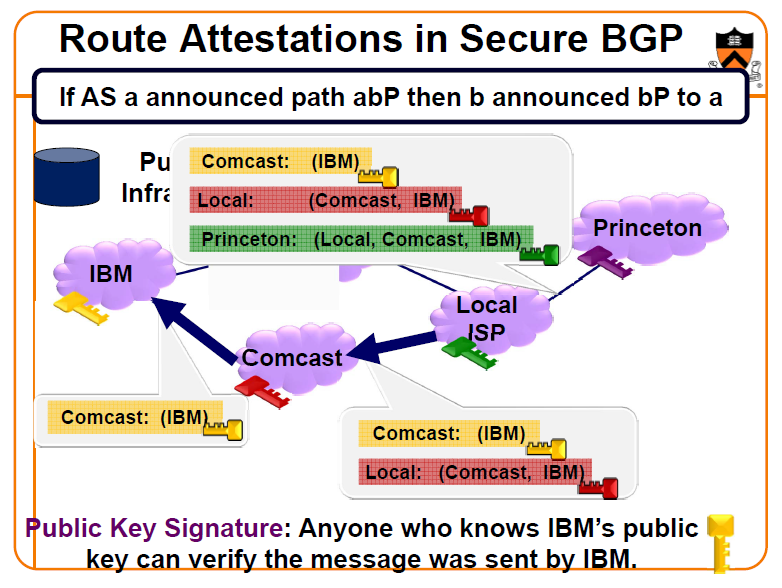
\includegraphics[scale = 0.6]{S-BGP.png}
 \end{figure}

There are two classes of attestations, address and route, although a single format is employed
to represent both. Route attestations are carried in a new type of
optional BGP path attribute as part of UPDATE messages.
\begin{itemize}
\item
\textbf{Address attestations} Here the issuer is the organization
that owns the address space and the subject is an AS that
may originate it, e.g., the organization's provider. The issuer signs an address attestation using the private key that
corresponds to the public key in the certificate.
assigning this address space to the issuer.
\item \textbf{Route attestations} Here the subject is a transit AS. A route
attestation is signed by the S-BGP speaker (or offline by
the management of the AS). The signer uses the private
key that corresponds to the public key in the certificate
that binds the speaker to the subject AS.
If an organization has more than one AS, there are separate attestations for each AS rather than just one attestation containing
multiple AS numbers. Each AS will have its own set of BGP
speakers and its own authentication certificate(s) as well. This
applies to both the stub and transit AS cases. Figure 3 summarizes the structure for address and route attestations.
\end{itemize}
\paragraph*{Route Validation}
Attestations and certificates are used by BGP speakers to validate routes asserted in UPDATE messages, i.e., to verify that
the first AS in the route has been authorized to advertise the address block(s) by the address block owner(s), and that each subsequent AS has been authorized to advertise the route for the
address block(s) by the preceding AS in the route. To validate a
route received from $AS_n,$, $AS_{n+1}$ needs:
\begin{itemize}
\item 1 address attestation from each organization owning an
address block or blocks in the NLRI
\item 1 address allocation certificate from each organization
owning an address block or blocks in the NLRI
\item 1 route attestation from every S-BGP speaker (or its AS)
along the path ( $AS_n$ to $AS_1$ ), where the route attestation
generated and signed by router$_x$ (or $AS_x$) specifies the
NLRI and the AS\_PATH from through
\item 1 certificate for each S-BGP speaker along the path ($AS_n$
to $AS_1$ ) to check the signatures on the route attestations
\end{itemize}
and, of course, all the relevant CRL’s must have been verified.

This means that, for each UPDATE, there must be attestations
confirming that all the ASes in the BGP UPDATE are authorized
to advertise routes to the destination IP address block(s). This
includes ASes that are providing third party advertisements for
ASes that are not running BGP.

The above elements allow the recipient of an 
UPDATE message by a BGP speaker to verify :
\begin{itemize}
\item An AS's authorization to “advertise” a block of addresses.
\item An organization's ownership of an AS number. 
\item An AS's identity. 
\item A BGP speaker's identity and its association with an AS.
\item Identity and authorization of a BGP peer. 
\item The AS represented by
that speaker the advertises
itself as the starting point of the route for the address prefix in the message, is the subject of an address attestation signed by
the owner of the address prefix.
\item For each AS in the route advertised in the message, that the signing BGP speaker is authorized to advertise to its neighbor the route constructed thus far, by the organization
owning the AS (in which the speaker resides).  
\end{itemize}
Moreover usage of IPSec ESP mode with IKE prevents replay of messages across a link, and
protects TCP against various forms of attack, including SYN
flooding and spoofed RSTs (resets).
\paragraph*{Distribution of Certificates and Attestations}
This architecture uses out-of-band distribution of certificates, CRL’s and address attestations to all S-BGP speakers. 

The alternative would be to transmit certificates as part of each UPDATE. This would ensure that each receiving BGP speaker would receive all the data needed to validate the route attestations in an UPDATE, and it would be easy
for each BGP speaker to include its own certificate as part of
the forwarding process. However, this would be very wasteful of
bandwidth, as each BGP speaker would receive many redundant
copies of certificates. More importantly, this approach is infeasible, because BGP UPDATE’s are limited in length to 4096
bytes and thus are too small to carry the necessary certificates
for most UPDATE’s.
The introduction of a new type of BGP
message for transmission of certificates (and CRL’s) could address the packet size problem, but would still tend to be very
wasteful of bandwidth and would not be backward compatible. 

Distribution happens in two tiers
of repositories from which one can download the entire certificate and CRL database. The top tier consists of several replicated, easy-to-access storage sites, e.g., the NAP route servers.
The second tier of repositories are operated by the ISP’s/DSP’s,
to provide local access for the S-BGP speakers within each
AS.

Route attestations are
distributed with BGP UPDATE’s in a newly defined, optional,
transitive path attribute. This approach requires BGP speakers
to be upgraded to a BGP release with these countermeasures.

\section{SSL/TLS}
The SSL Record Protocol provides basic security services to various higher-layer protocols. In particular, the Hypertext Transfer Protocol (HTTP), which provides the transfer service for Web client/server interaction, can operate on top of SSL. Three higher-layer protocols are defined as part of SSL: the Handshake Protocol, The Change Cipher Spec Protocol, and the Alert Protocol. 

Two important SSL concepts are the SSL session and the SSL connection, which are defined in the specification as follows:
\begin{description}
\item[Connection] A connection is a transport (in the OSI layering model definition) that provides a suitable type of service. For SSL, such connections are peer-to-peer relationships. The connections are transient. Every connection is associated with one session.
\item[Session] An SSL session is an association between a client and a server. Sessions are created by the Handshake Protocol. Sessions define a set of cryptographic security parameters, which can be shared among multiple connections. Sessions are used to avoid the expensive negotiation of new security parameters for each connection.
\end{description}
Between any pair of parties (applications such as HTTP on client and server), there may be multiple secure connections. In theory, there may also be multiple simultaneous sessions between parties, but this feature is not used in practice.

There are actually a number of states associated with each session. Once a session is established, there is a current operating state for both read and write (i.e., receive and send). In addition, during the Handshake Protocol, pending read and write states are created. Upon successful conclusion of the Handshake Protocol, the pending states become the current states.
A session state is defined by the following parameters:
\begin{itemize}

\item Session identifier: An arbitrary byte sequence chosen by the server to identify an active or resumable session state.
\item Peer certificate: An X509.v3 certificate of the peer. This element of the state may be null.
\item Compression method: The algorithm used to compress data prior to encryption.
\item Cipher spec: Specifies the bulk data encryption algorithm (such as null, AES, etc.) and a hash algorithm (such as MD5 or SHA-1) used for MAC calculation. It also defines cryptographic attributes such as the hash\_size.
\item Master secret: 48-byte secret shared between the client and server.
\item Is resumable: A flag indicating whether the session can be used to initiate new connections.
\end{itemize}
A connection state is defined by the following parameters:
\begin{itemize}
\item Server and client random: Byte sequences that are chosen by the server and client for each connection.
\item Server write MAC secret: The secret key used in MAC operations on data sent by the server.
\item Client write MAC secret: The secret key used in MAC operations on data sent by the client.
\item Server write key: The conventional encryption key for data encrypted by the server and
decrypted by the client.
\item Client write key: The conventional encryption key for data encrypted by the client and
decrypted by the server.
\item Initialization vectors: When a block cipher in CBC mode is used, an initialization vector (IV) is
maintained for each key. This field is first initialized by the SSL Handshake Protocol. Thereafter the final ciphertext block from each record is preserved for use as the IV with the following record.
\item Sequence numbers: Each party maintains separate sequence numbers for transmitted and received messages for each connection. When a party sends or receives a change cipher spec message, the appropriate sequence number is set to zero. Sequence numbers may not exceed $2^{64}-1$.
\end{itemize}

The SSL Record Protocol provides two services for SSL connections:
\begin{description}
\item[Confidentiality] The Handshake Protocol defines a shared secret key that is used for conventional encryption of SSL payloads.
\item[Message Integrity] The Handshake Protocol also defines a shared secret key that is used to form a message authentication code (MAC).
\end{description}
\subsection{SSL Record Protocol Operation}
This operation has the following steps:
\begin{enumerate}
\item The first step is \textbf{fragmentation}. Each upper-layer message is fragmented into blocks of $2^{14}$ bytes (16384 bytes) or less.
\item Next, \textbf{compression} is optionally applied. Compression must be lossless and may
not increase the content length by more than 1024 bytes. In SSLv3 (as well as the current version of TLS), no compression algorithm is specified, so the default compression algorithm is null.
\item The next step in processing is to compute a \textbf{message authentication code} over the compressed data. For this purpose, a shared secret key is used. The calculation is defined as:
\begin{verbatim}
hash(shared secret key || pad_2 ||
      hash(MAC_write_secret || pad_1 || seq_num ||
      SSLCompressed.type ||
      SSLCompressed.length || SSLCompressed.fragment))
\end{verbatim}
where $hash$ is either MD5 or SHA-1, $pad_2$ is the byte 0x5C (0101 1100) repeated 48 times for MD5 and 40 times for SHA-1 and $pad_1$ is the byte 0x36 (0011 0110) repeated 48 times (384 bits) for MD5 and 40 times (320 bits) for SHA-1.
\item Next, the compressed message plus the MAC are \textbf{encrypted} using symmetric encryption. Encryption may not increase the content length by more than 1024 bytes, so that the total length may not exceed $2^{14}$ + 2048.
\item The final step of SSL Record Protocol processing is to prepend a \textbf{header}, consisting of the following fields:
\begin{itemize}
\item Content Type (8 bits): The higher layer protocol used to process the enclosed fragment. The content types that have been defined are change\_cipher\_spec, alert, handshake, and application\_data.  
\item Major Version (8 bits): Indicates major version of SSL in use. For SSLv3, the value is 3.
\item Minor Version (8 bits): Indicates minor version in use. For SSLv3, the value is 0.
\item Compressed Length (16 bits): The length in bytes of the plaintext fragment (or compressed fragment if compression is used). The maximum value is $2^{14}$ + 2048.
\end{itemize}
\end{enumerate}

\subsection{Change Cipher Spec Protocol}
The Change Cipher Spec Protocol is one of the three SSL-specific protocols that use the SSL Record Protocol, and it is the simplest. This protocol consists of a single message which consists of a single byte with the value 1. The sole purpose of this message is to cause the pending state to be copied into the current state, which updates the cipher suite to be used on this connection.
\subsection{Alert Protocol}
The Alert Protocol is used to convey SSL-related alerts to the peer entity. As with other applications that use SSL, alert messages are compressed and encrypted, as specified by the current state.
Each message in this protocol consists of two bytes. The first byte takes the value
warning(1) or fatal(2) to convey the severity of the message. If the level is fatal, SSL immediately terminates the connection. Other connections on the same session may continue, but no new connections on this session may be established. The second byte contains a code that indicates the specific alert. 

Fatal alerts include \textit{unexpected\_message, bad\_record\_mac, decompression\_failure, handshake\_failure and illegal\_parameter. } 
The remainder of the alerts are 
\textit{close\_notify,
no\_certificate,
bad\_certificate, unsupported\_certificate,
certificate\_revoked,
certificate\_expired} and
\textit{certificate\_ unknown}.

\subsection{Handshake Protocol}
The most complex part of SSL is the Handshake Protocol. This protocol allows the server and client to authenticate each other and to negotiate an encryption and MAC algorithm and cryptographic keys to be used to protect data sent in an SSL record. The Handshake Protocol is used before any application data is transmitted.

There are four main phases in the Handshake protocol:
\begin{description}
\item[1. Establish Security Capabilities]
This phase is used to initiate a logical connection and to establish the security capabilities that will be associated with it. The exchange is initiated by the client, which sends a\textbf{ client\_hello message} with the following parameters: 
\begin{itemize}
\item Version: The highest SSL version understood by the client.
\item Random: A client-generated random structure, consisting of a 32-bit timestamp and 28 bytes generated by a secure random number generator. These values serve as nonces and are used
during key exchange to prevent replay attacks.
\item Session ID: A variable-length session identifier. A nonzero value indicates that the client wishes
to update the parameters of an existing connection or create a new connection on this session. A zero value indicates that the client wishes to establish a new connection on a new session.
\item CipherSuite: This is a list that contains the combinations of cryptographic algorithms supported
by the client, in decreasing order of preference. Each element of the list (each cipher suite)
defines both a key exchange algorithm and a CipherSpec; these are discussed subsequently.
\item Compression Method: This is a list of the compression methods the client supports.
\end{itemize}
After sending the client\_hello message, the client waits for the \textbf{server\_hello message}, which contains the same parameters as the client\_hello message.
\item[2. Server Authentication and Key Exchange]
The server begins this phase by sending its \textbf{certificate}, if it needs to be authenticated; the message contains one or a chain of X.509 certificates. The certificate message is required for any agreed-on key exchange method except anonymous Diffie-Hellman. Note that if fixed Diffie-Hellman is used, this certificate message functions as the server's key exchange message because it contains the server's public Diffie-Hellman parameters.

Next, a \textbf{server\_key\_exchange} message may be sent if it is required. It is not required in two instances: (1) The server has sent a certificate with fixed Diffie-Hellman parameters, or (2) RSA key exchange is to be used. 

Some further details about the signatures are warranted. As usual, a signature is created by taking the
hash of a message and encrypting it with the sender's private key. In this case the hash is defined as
\begin{verbatim}
hash(ClientHello.random || ServerHello.random || ServerParams)
\end{verbatim}
So the hash covers not only the Diffie-Hellman or RSA parameters, but also the two nonces from the initial hello messages. This ensures against replay attacks and misrepresentation. In the case of a DSS signature, the hash is performed using the SHA-1 algorithm. In the case of an RSA signature, both an MD5 and an SHA-1 hash are calculated, and the concatenation of the two hashes (36 bytes) is encrypted with the server's private key.

Next, a non-anonymous server (server not using anonymous Diffie-Hellman) can request a \textbf{certificate} from the client. The certificate\_request message includes two parameters: certificate\_type and certificate\_authorities.

The final message in Phase 2, and one that is always required, is the \textbf{server\_done} message, which is sent by the server to indicate the end of the server hello and associated messages. After sending this message, the server will wait for a client response. This message has no parameters.
\item[3. Client Authentication and Key Exchange]
Upon receipt of the server\_done message, the client should verify that the server provided a valid certificate if required and check that the server\_hello parameters are acceptable. If all is satisfactory, the client sends one or more messages back to the server.

If the server has requested a certificate, the client begins this phase by sending a certificate message. If no suitable certificate is available, the client sends a \textbf{no\_certificate} alert instead.
Next is the \textbf{client\_key\_exchange} message, which must be sent in this phase. The content of the message depends on the type of key exchange.

Finally, in this phase, the client may send a \textbf{certificate\_verify} message to provide explicit verification of a client certificate. This message is only sent following any client certificate that has signing capability (i.e., all certificates except those containing fixed Diffie-Hellman parameters). The purpose is to verify the client's ownership of the private key for the client certificate. Even if someone is misusing the client's certificate, he or she would be unable to send this message.
\item[4. Finish]
This phase completes the setting up of a secure connection. The client sends a \textbf{change\_cipher\_spec} message and copies the pending CipherSpec into the current CipherSpec. Note that this message is not considered part of the Handshake Protocol but is sent using the Change Cipher Spec Protocol. The client then immediately sends the \textbf{finished} message under the new algorithms, keys, and secrets. The finished message verifies that the key exchange and authentication processes were successful. The content of the finished message is the concatenation of two hash values:
\begin{verbatim}
MD5(master_secret || pad2 || MD5(handshake_messages ||
    Sender || master_secret || pad1))    
\end{verbatim}
or
\begin{verbatim}
SHA(master_secret || pad2 || SHA(handshake_messages ||
    Sender || master_secret || pad1))
\end{verbatim}

where \textit{Sender} is a code that identifies that the sender is the client and \textit{handshake\_messages} is all of the data from all handshake messages up to but not including this message.
In response to these two messages, the server sends its own \textbf{change\_cipher\_spec} message, transfers the pending to the current CipherSpec, and sends its \textbf{finished} message. At this point the handshake is complete and the client and server may begin to exchange application layer data.
\begin{figure}[h!]
  \centering
  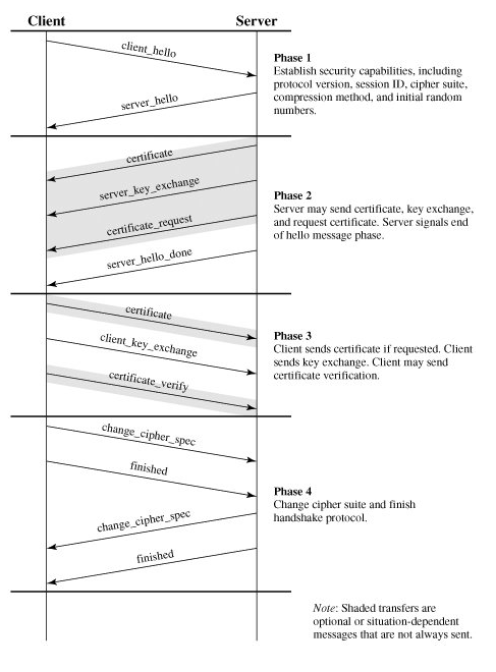
\includegraphics[scale = 0.8]{SSL-Handshake.png}
  \caption{SSL Handshake Protocol}
 \end{figure}
\end{description}
\subsection{Transport Layer Security}
TLS is an IETF standardization initiative whose goal is to produce an Internet standard version of SSL. It is very similar to SSLv3 except fot the following differences.


\paragraph*{Version Number}
The TLS Record Format is the same as that of the SSL Record Format and the fields in the header have the same meanings. The one difference is in version values. For the current version of TLS, the Major Version is 3 and the Minor Version is 1.
\paragraph*{Message Authentication Code}
There are two differences between the SSLv3 and TLS MAC schemes: the actual algorithm and the scope of the MAC calculation. TLS makes use of the \textbf{HMAC} algorithm defined in RFC 2104. 
$$ HMAC_K(M) = H[K^+ \oplus pad_1 || K^+ \oplus pad_2 || M]$$ where $H$ is the designated hash function (MD5 or SHA-1), $M$ is  message input to HMAC and$K^+$ is the
secret key padded with zeros on the left so that the result is equal to the block length of the hash code(for MD5 and SHA-1, block length = 512 bits)

SSLv3 uses the same algorithm, except that the padding bytes are concatenated with the secret key rather than being XORed with the secret key padded to the block length. The level of security should be about the same in both cases.

For TLS, the MAC calculation encompasses the fields indicated in the following expression:

\begin{verbatim}
 HMAC_hash(MAC_write_secret, seq_num || TLSCompressed.type ||
          TLSCompressed.version || TLSCompressed.length ||
          TLSCompressed.fragment)       
\end{verbatim}
The MAC calculation covers all of the fields covered by the SSLv3 calculation, plus the field TLSCompressed.version, which is the version of the protocol being employed.
\paragraph*{Pseudorandom Function}
TLS makes use of a pseudorandom function referred to as PRF to expand secrets into blocks of data for purposes of key generation or validation. The objective is to make use of a relatively small shared secret value but to generate longer blocks of data in a way that is secure from the kinds of attacks made on hash functions and MACs. The PRF is based on the following data expansion function:

\begin{verbatim}
P_hash(secret, seed) = HMAC_hash(secret, A(1)  || seed) ||
                       HMAC_hash(secret, A(2)  || seed) ||
                       HMAC_hash(secret, A(3) || seed) || ...
                       
\end{verbatim}
where A() is defined as:
\begin{align*}
A(0) &= seed\\
A(i) &= HMAC_{hash }(secret, A(i - 1))
\end{align*}
The data expansion function makes use of the HMAC algorithm, with either MD5 or SHA-1 as the underlying hash function. As can be seen, P\_hash can be iterated as many times as necessary to produce the required quantity of data. For example, if P\_SHA-1 was used to generate 64 bytes of data, it would have to be iterated four times, producing 80 bytes of data, of which the last 16 would be discarded. In this case, P\_MD5 would also have to be iterated four times, producing exactly 64 bytes of data. Note that each iteration involves two executions of HMAC, each of which in turn involves two executions of the underlying hash algorithm.

To make PRF as secure as possible, it uses two hash algorithms in a way that should guarantee its security if either algorithm remains secure. PRF is defined as
\begin{verbatim}
PRF(secret, label, seed) = P_MD5(S1, label || seed)
                           P_SHA-1(S2, label || seed)              
\end{verbatim}

PRF takes as input a secret value, an identifying label, and a seed value and produces an output of arbitrary length. The output is created by splitting the secret value into two halves (S1 and S2) and performing P\_hash on each half, using MD5 on one half and SHA-1 on the other half. The two results are XORed to produce the output; for this purpose, P\_MD5 will generally have to be iterated more times than P\_SHA-1 to produce an equal amount of data for input to the XOR function.
\paragraph*{Certificate\_Verify and Finished Messages}
In the TLS certificate\_verify message, the MD5 and SHA-1 hashes are calculated only over handshake\_messages. Recall that for SSLv3, the hash calculation also included the master secret and pads. These extra fields were felt to add no additional security.
As with the finished message in SSLv3, the finished message in TLS is a hash based on the shared master\_secret, the previous handshake messages, and a label that identifies client or server. The calculation is somewhat different. For TLS, we have
\begin{verbatim}
PRF(master_secret, finished_label, MD5(handshake_messages)||
    SHA-1(handshake_messages))

\end{verbatim}
where finished\_label is the string "client finished" for the client and "server finished" for the server.
\paragraph*{Padding}
In SSL, the padding added prior to encryption of user data is the minimum amount required so that the total size of the data to be encrypted is a multiple of the cipher's block length. In TLS, the padding can be any amount that results in a total that is a multiple of the cipher's block length, up to a maximum of 255 bytes. For example, if the plaintext (or compressed text if compression is used) plus MAC plus padding.length byte is 79 bytes long, then the padding length, in bytes, can be 1, 9, 17, and so on, up to 249. A variable padding length may be used to frustrate attacks based on an analysis of the lengths of exchanged messages.
\paragraph*{Other Minor Changes}
TLS includes some additional Alert codes, does not accomodate the Fortezza algorithm for key exchange or encryption and the computation of secret key and block key (if necessary) is somewhat different from SSL.

\section{DNSsec}
\subsection*{DNS Overview}
DNS is a global, hierarchical and distributed database. This database associates names, which
are referred to as domain names, with certain data containedin resource records (RRs). Records linked to a domain name can be of different types, but the address type is the most
common one. There can be multiple RRs of the same type
for one domain name. The set of resource records of the
same type is called a resource record set (RRset).
Since domain names need to be globally unique, a hierar-
chical naming scheme is used. A domain name refers to a
node in a tree which is called the domain name
space. Each subtree is called a
domain. For example, the subtree rooted on the .com node
is called the .com domain and includes all domain names
ending with .com. The nodes that are direct children of the
root node are called top level domains.

Communication with the DNS database follows the client/
server paradigm. The domain name tree is divided into
zones, which usually are contiguous parts of the tree. Zones
are defined by the process of delegation which assigns to
some organization the responsibility of managing particular
subdomains. A zone may contain information about a domain and its subdomains. Top-level zones, such as .edu,
would mostly contain delegation information.
For each zone, there are authoritative servers (name servers)
answering all queries concerning domain names in that zone.
Name servers can be authoritative for multiple zones, too.
A DNS client program is called a resolver. 

Root servers are essential to the functionality of the DNS
system. There are currently 13 root DNS servers distributed
all over the planet. Caching techniques are employed to
reduce the number of requests in order to speed up the process resolving and to reduce network traffic. Consequently,
each RR that is returned from a DNS server has a certain
time-to-live (TTL) which is the time the RR can be cached.
\begin{figure}[h!]
        \centering
        \begin{subfigure}[b]{0.45\textwidth}
                \centering
                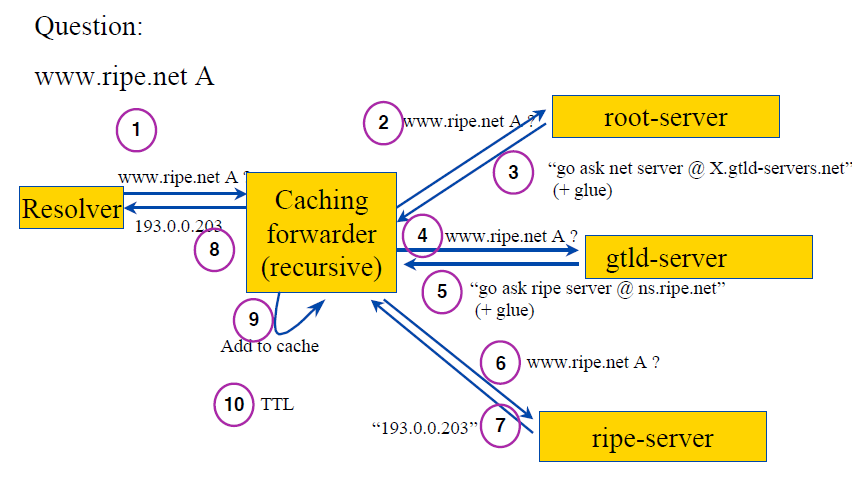
\includegraphics[width=\textwidth]{DNS.png}
                \caption{DNS}
                \end{subfigure}
        \qquad
        \begin{subfigure}[b]{0.45\textwidth}
                \centering
                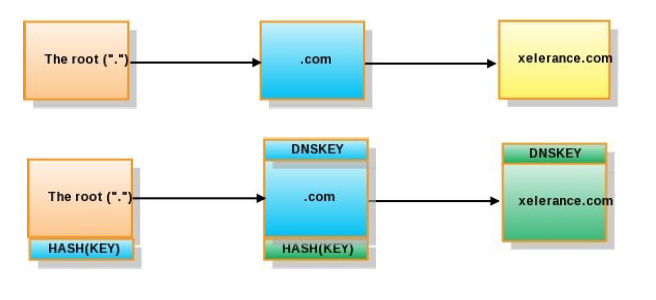
\includegraphics[width=\textwidth]{DNSSec.png}
                \caption{DNSSec}
                \end{subfigure}
       \end{figure}
\subsection{DNSsec Overview}
The primary goal of DNSSEC is to provide authentication and integrity for data received from the DNS database.
This is done via digital signature schemes based on public-
key cryptography. A possible approach is to sign each DNS
message. The general idea is that each node in the DNS tree
is associated with a public key of some sort. Each message
from DNS servers is signed under the corresponding private-
key. 
\begin{figure}[h!]
  \centering
  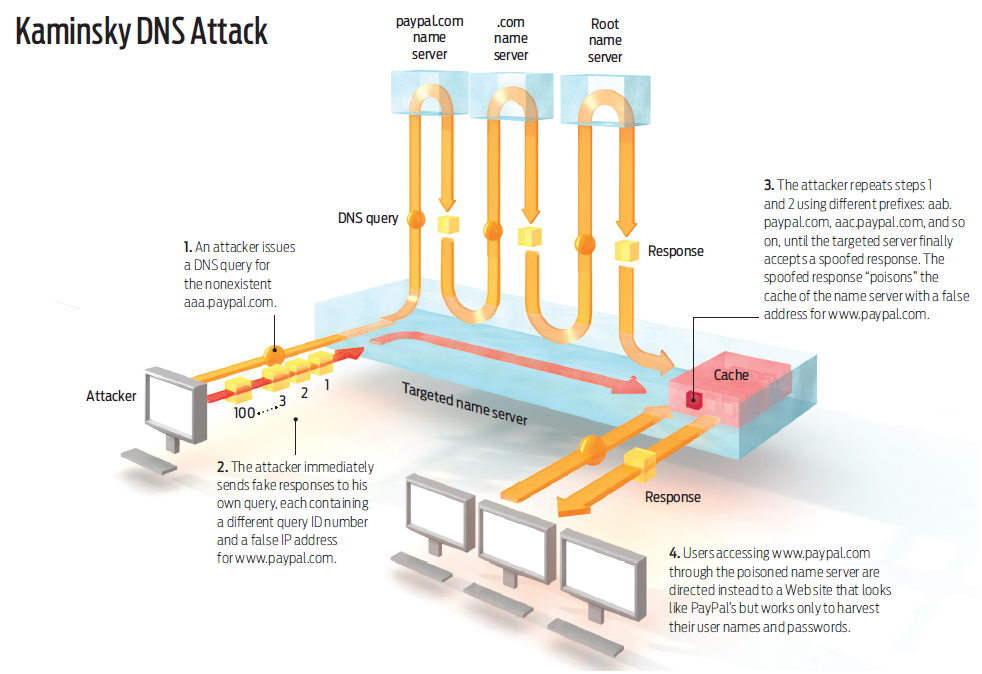
\includegraphics[scale = 0.5]{Kaminsky.png}
\end{figure}

It is assumed that one or more authenticated DNS root
public keys are publicly known. These keys are used to
generate certificates on behalf of the top level domains, i.e.
these keys are used to generate a signature that binds the
identity information of each top-level domain to the corresponding public key. The top level domains sign the keys of
their subdomains and so on in a process where each parent
signs the public keys of all its children in the DNS tree. A resolver, that owns an
authentic copy of the root's public key, will receive the IP
address of the DNS server of .com from the root along with
its public key all signed via a pre-specified digital signature
algorithm. The public key for the .com zone is trusted since
it is signed by the root and will be used to sign the public
key of the DNS server of lab.com. This process is repeated
going down across the tree. To associate a domain name with a certain public key, a so called KEY RR is used.

Currently, DSA and RSA are the digital signature
algorithms supported by DNSSEC. The Diffie-Hellman key
agreement protocol is also supported.
Two different kinds of signatures for DNS messages as a
whole are currently defined: transaction signatures (TSIGs) based on symmetric techniques, and public-key signatures which are abbreviated by SIG(0). TSIG signatures have been introduced mainly for transactions between
local servers, for instance between the resolver and the stub
resolver. It is convenient to use TSIG to secure dynamic
updates or zone transfers between master and slave servers.
SIG(0) is similar to TSIG but employs public-key signatures.
SIG(0) may not be practical to use on a large scale but it
is useful in case integrity protection and authentication of
the message as a whole are desired. SIG(0) could be used to
authenticate requests when it is necessary to check whether
the requester has some required privilege.
A more efficient alternative employs digital signatures to
sign each RRset. The basic idea is to
cover each resource record set with a public-key signature
which is stored as a resource record called SIG RR.
These SIG RRs are computed for every RRset in a zone file
and stored therein. A DNS server adds the corresponding
pre-calculated signature for each RRset in answers to DNS
queries. It is imperative for DNS servers to include the entire
RRset in a DNS answer as otherwise the resolver could not
verify the signature.

For this scheme it is also necessary to introduce an additional type of resource records: NXT RRs [20]. The NXT
resource record is associated with a domain name and in-
dicates the types of RRs that are available for that domain
name and additionally which domain name is next by dic-
tionary order (the zone should be in canonical order). In
order to build a closed chain of NXT records for a zone,
the first and the last entry are considered to be next to
each other. These NXT resource records are, like any other
RRset, signed. If a resolver queries for a domain name or
a type of data that does not exist, the corresponding NXT
RR and a covering SIG RR are returned. The NXT records
identify what does not exist in a zone to avoid generating sig-
natures on general statements of nonexistence which could
be replayed. However, notice that an attacker could query
for the NXT record of a domain name to and the next domain name in canonical order and repeat the process to learn
all the domain names in the zone.

\end{document}
